\section{Exercise 1}
Cho sơ đồ mạch điện sau. Tính giá trị của $v_0$ và $i$. Sau đó mô phỏng mạch để kiểm tra kết quả
\begin{figure}[!htbp]
    \centering
    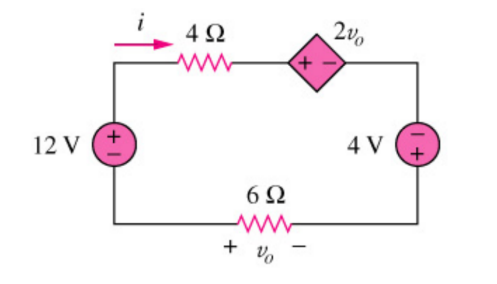
\includegraphics[width=0.5\textwidth]{graphics/ex1/f1.PNG}
    \caption{}
\end{figure}

\subsection{Tính toán}

Áp dụng KVL cho loop theo chiều kim đồng hồ, ta có:
\begin{align}
    -12 + 4i +2v_0 - 4 + 6i = 0
\end{align}
Áp dụng định luật Ohm cho điện trở $6 \Omega$
\begin{align}
    v_0 = -6i
\end{align}
Từ (1.1) và (1.2), ta được:
\begin{align*}
    -16 + 10i - 12i = 0 \rightarrow i = -8 \ \text{A}
\end{align*}
và \(v_0 = 48 \ \text{V}\)

\subsection{Mô phỏng}

Kết quả mô phỏng:

\begin{figure}[!htbp]
    \centering
    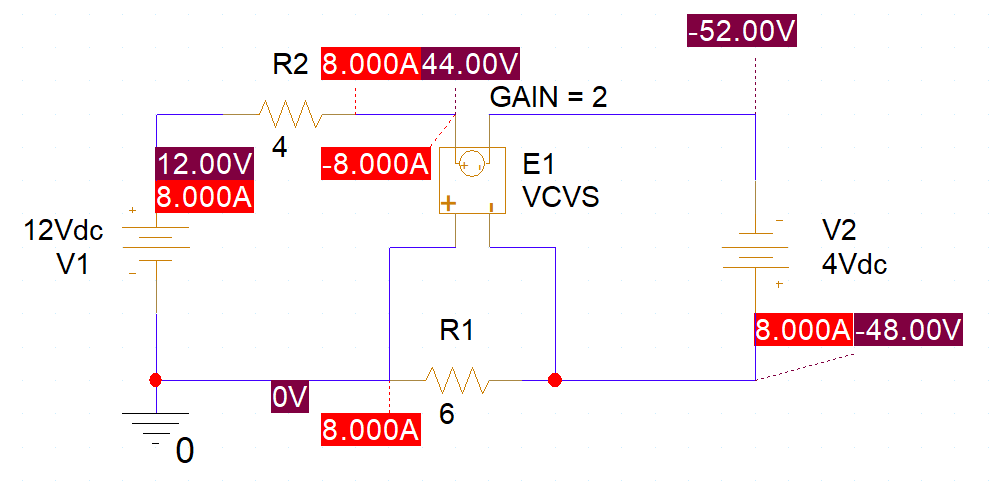
\includegraphics[width=0.7\textwidth]{graphics/ex1/f2.PNG}
\end{figure}